% plots.tex — a small gallery of plots for Dana (2D functions + 3D surfaces).
% Compile:  scripts/tex2pdf.sh scripts/plots.tex   ->  generated-latex/plots.pdf
\documentclass[11pt]{article}
\usepackage[margin=1in]{geometry}
\usepackage{amsmath}
\usepackage{pgfplots}
\pgfplotsset{compat=1.18}

\title{Plots}
\author{ScottLean4 \textperiodcentered\ for Dana Scott}
\date{}

\begin{document}
\maketitle

\section*{Two functions}
\begin{center}
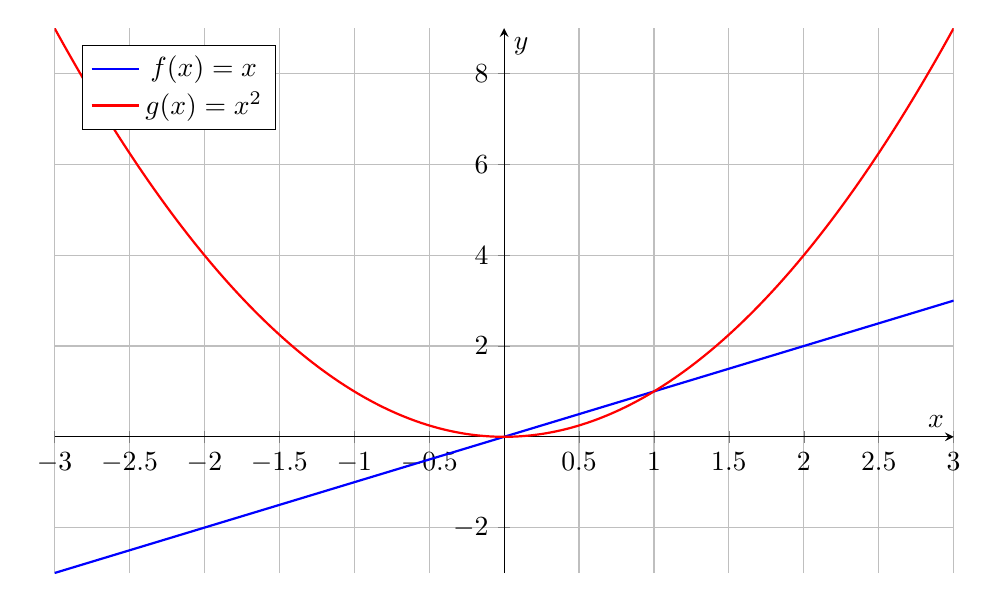
\begin{tikzpicture}
  \begin{axis}[axis lines=middle, xlabel=$x$, ylabel=$y$,
      domain=-3:3, samples=200, grid=both,
      width=13cm, height=8.5cm, legend pos=north west]
    \addplot[blue, thick] {x};   \addlegendentry{$f(x)=x$}
    \addplot[red,  thick] {x^2}; \addlegendentry{$g(x)=x^2$}
  \end{axis}
\end{tikzpicture}
\end{center}

\newpage
\section*{Two surfaces}
\begin{center}
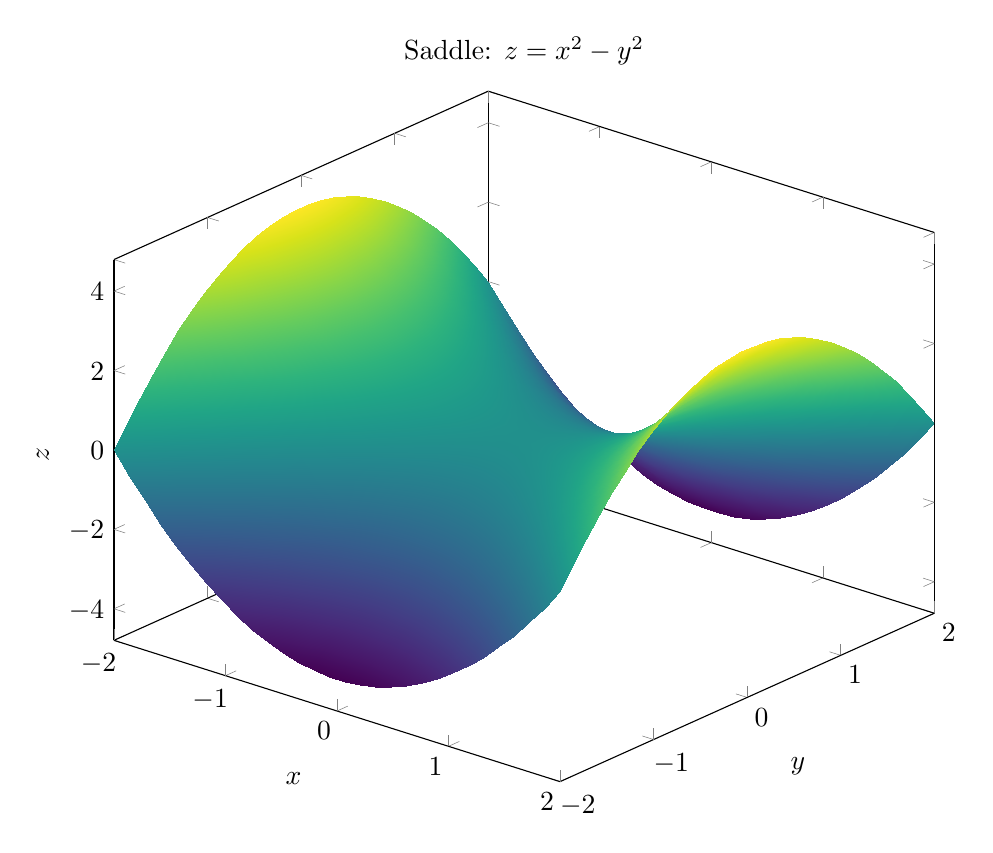
\begin{tikzpicture}
  \begin{axis}[title={Saddle: $z = x^2 - y^2$}, width=12cm, view={40}{30},
      colormap/viridis, xlabel=$x$, ylabel=$y$, zlabel=$z$]
    \addplot3[surf, shader=interp, samples=30, domain=-2:2, y domain=-2:2] {x^2 - y^2};
  \end{axis}
\end{tikzpicture}

\vspace{1.2em}

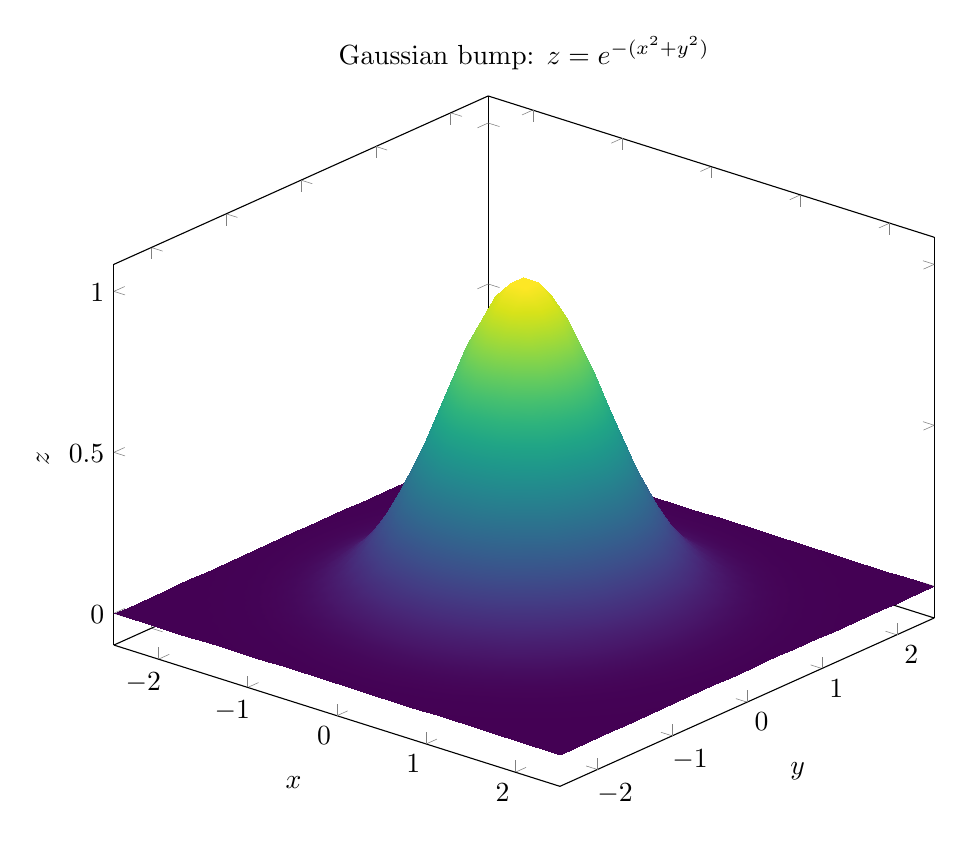
\begin{tikzpicture}
  \begin{axis}[title={Gaussian bump: $z = e^{-(x^2+y^2)}$}, width=12cm, view={40}{30},
      colormap/viridis, xlabel=$x$, ylabel=$y$, zlabel=$z$]
    \addplot3[surf, shader=interp, samples=30, domain=-2.5:2.5, y domain=-2.5:2.5]
      {exp(-(x^2+y^2))};
  \end{axis}
\end{tikzpicture}
\end{center}

\end{document}
